\documentclass[10pt,letterpaper]{article}
\usepackage[
    lmargin=2.2in,
    rmargin=0.7in,
    tmargin=1.0in,
    bmargin=1.0in
]{geometry}
\usepackage{notes}
\usepackage{pgfplots}
\pgfplotsset{compat=1.18}

% Shared figure styles. Arrows on trajectories always show increasing time.
\definecolor{curve}{HTML}{247E91}
\tikzset{
    orbit/.style={black,thick},
    inward/.style={blue,very thick},
    outward/.style={red,very thick}
}
\newcommand{\phaseaxes}{%
    \draw[->,gray](-3.25,0)--(3.45,0)node[right]{$x$};
    \draw[->,gray](0,-3.25)--(0,3.45)node[above]{$y$};
}
% Argument -1 gives inward motion, +1 outward motion.
\newcommand{\noderays}[1]{%
    \ifnum#1<0\def\raystyle{inward}\else\def\raystyle{outward}\fi
    \draw[\raystyle](-3.1,0)--(3.1,0);
    \draw[\raystyle](0,-3.1)--(0,3.1);
    \foreach \s in {-1,1}{
        \draw[->,\raystyle]({\s*(1.3-.4*#1)},0)--({\s*(1.3+.4*#1)},0);
        \draw[->,\raystyle](0,{\s*(1.3-.4*#1)})--(0,{\s*(1.3+.4*#1)});
    }
    \fill(0,0)circle(2pt);
}
\newcommand{\nodecurves}[1]{%
    \foreach \sx in {-1,1}{\foreach \c in {-.9,-.25,.25,.9}{
        \pgfmathsetmacro{\endx}{min(3.1,sqrt(3.1/abs(\c)))}
        \draw[orbit]plot[domain=.02:\endx,samples=100]({\sx*\x},{\c*\x*\x});
        \pgfmathsetmacro{\fromx}{1-.18*#1}
        \pgfmathsetmacro{\tox}{1+.18*#1}
        \draw[->,orbit]plot[domain=\fromx:\tox,samples=20]({\sx*\x},{\c*\x*\x});
    }}
}

\begin{document}
\begin{center}
\Large\textbf{DAY 32 -- Nodes, Stability, and a Line of Equilibria}\\
\normalsize (Section 4.4.1)
\end{center}

\section{From Saddles to Nodes}

% SIDE NOTE: 9:00 | Pick up after the tilted saddle
% a) Recall eigenvectors give the lines; eigenvalue signs give the arrows.
% b) Ask how the four arrows change when both eigenvalues are negative.
% c) Do not repeat the full linear-orbit construction.

Last time, we sketched linear orbits and used them to sketch saddles,
including saddles with tilted eigenvector lines. Today, we use the same
starting point to sketch nodes, then describe stability and what changes
when an eigenvalue is zero.

For two distinct real, nonzero eigenvalues,
\[
\mathbf{x}(t)=c_1e^{\lambda_1t}\mathbf{v}_1+c_2e^{\lambda_2t}\mathbf{v}_2.
\]
The eigenvectors give two lines containing four linear orbits.
The sign of each eigenvalue determines motion along its rays:
\[
\lambda<0:\ \text{inward},\qquad \lambda>0:\ \text{outward}.
\]
Opposite signs give a \textbf{saddle point}. When the eigenvalues have
the same sign, the origin is a \textbf{node}. The new question is how
the curved trajectories fit between the linear orbits.

\section{Sketching Nodes}

% SIDE NOTE: 9:03 | First node: four rays, then one curve
% a) Use the diagonal eigenpairs directly; all four rays point inward.
% b) Apply (1,1), eliminate time, and draw the right half of the parabola.
% c) Skip deriving the general coefficient formula if needed; finish by 9:11.
\subsection{Both Eigenvalues Negative}
When two distinct real eigenvalues have the same sign, the origin is a
\textbf{node}. We again begin with the linear orbits and then study the
curves between them.
\begin{example}[1]{
For the system
\[
\mathbf{x}'=\begin{pmatrix}-1&0\\0&-2\end{pmatrix}\mathbf{x},
\]
sketch the linear orbits, find the solution with $\mathbf{x}(0)=(1,1)^T$,
and use its trajectory to complete the phase portrait.
}
The general solution is
\[
\mathbf{x}(t)=c_1e^{-t}\begin{pmatrix}1\\0\end{pmatrix}
+c_2e^{-2t}\begin{pmatrix}0\\1\end{pmatrix}.
\]
\paragraph{Step 1. Draw the linear orbits.}
The eigenvector lines are the coordinate axes. Both eigenvalues are negative,
so all four rays point toward the origin.

\paragraph{Step 2. Find one curved trajectory.}
The initial condition gives $c_1=c_2=1$, so
\[
\mathbf{x}(t)=\begin{pmatrix}e^{-t}\\e^{-2t}\end{pmatrix},
\qquad \boxed{y=x^2,\quad x>0.}
\]
The particle moves down and left along the parabola toward the origin.
It never reaches the origin at a finite time.
\begin{center}
\begin{minipage}[t]{.47\linewidth}\centering
\resizebox{.79\linewidth}{!}{\begin{tikzpicture}[>=Stealth]
\phaseaxes\noderays{-1}
\end{tikzpicture}}

\small First: four inward rays.
\end{minipage}\hfill
\begin{minipage}[t]{.47\linewidth}\centering
\resizebox{.79\linewidth}{!}{\begin{tikzpicture}[>=Stealth]
\phaseaxes\noderays{-1}
\draw[purple,very thick]plot[domain=.02:1.76,samples=80](\x,{\x*\x});
\draw[->,purple,very thick]plot[domain=1.3:.9,samples=20](\x,{\x*\x});
\fill[purple](1,1)circle(2pt)node[right]{$(1,1)$};
\end{tikzpicture}}

\small Then: one curved trajectory.
\end{minipage}
\end{center}
\paragraph{Step 3. Add curves in the other regions.}
For $c_1c_2\ne0$, eliminating $t$ gives
\[
 y=\frac{c_2}{c_1^2}x^2.
\]
Each curve stays in its region. The two halves of a parabola are separate
trajectories. Draw representative curves and orient them toward the origin.
\end{example}


% SIDE NOTE: 9:11 | Check the curves against the field
% a) At (1,1), velocity is (-1,-2).
% b) Trace the overlay toward the origin; notice the horizontal tangent.
% c) Show the prepared figures; skip drawing the grid or demonstrating MATLAB.
\subsection{Checking the Shape with a Direction Field}

For the system in Example 1,
\[
    x'=-x,\qquad y'=-2y,
\]
the velocity at a point $(x,y)$ is
\[
    \mathbf{x}'=
    \begin{pmatrix}-x\\-2y\end{pmatrix}.
\]
The direction field below helps us check the shapes
of our trajectories. The parabolic curves follow
the arrows and become tangent to the horizontal
axis as they approach the origin.

\begin{center}
%-------------------- Field alone --------------------
\begin{minipage}[t]{0.48\linewidth}
\centering
\begin{tikzpicture}[scale=0.48,>=Stealth]
    % Axes
    \draw[->,gray] (-3.5,0) -- (3.5,0)
        node[right,black] {$x$};
    \draw[->,gray] (0,-3.5) -- (0,3.5)
        node[above,black] {$y$};

    % Direction field: (-x,-2y)
    \foreach \xx in {-3,-2,-1,0,1,2,3}{
        \foreach \yy in {-3,-2,-1,0,1,2,3}{
            \pgfmathsetmacro{\fieldnorm}
                {sqrt(\xx*\xx+4*\yy*\yy)}
            \ifdim\fieldnorm pt>0pt
                \draw[->,gray!75,thick]
                    (\xx,\yy) --
                    ({\xx-0.45*\xx/\fieldnorm},
                     {\yy-0.90*\yy/\fieldnorm});
            \fi
        }
    }

    \fill (0,0) circle (2pt);
\end{tikzpicture}

\small Direction field.
\end{minipage}
\hfill
%-------------------- Field and trajectories --------------------
\begin{minipage}[t]{0.48\linewidth}
\centering
\begin{tikzpicture}[scale=0.48,>=Stealth]
    % Axes
    \draw[->,gray] (-3.5,0) -- (3.5,0)
        node[right,black] {$x$};
    \draw[->,gray] (0,-3.5) -- (0,3.5)
        node[above,black] {$y$};

    % Same direction field
    \foreach \xx in {-3,-2,-1,0,1,2,3}{
        \foreach \yy in {-3,-2,-1,0,1,2,3}{
            \pgfmathsetmacro{\fieldnorm}
                {sqrt(\xx*\xx+4*\yy*\yy)}
            \ifdim\fieldnorm pt>0pt
                \draw[->,gray!50,thick]
                    (\xx,\yy) --
                    ({\xx-0.45*\xx/\fieldnorm},
                     {\yy-0.90*\yy/\fieldnorm});
            \fi
        }
    }

    % Parabolic trajectories and inward orientation
    \begin{scope}
        \clip (-3.1,-3.1) rectangle (3.1,3.1);

        \foreach \sx in {-1,1}{
            \foreach \C in {-1,-0.3,0.3,1}{
                \draw[blue,thick,
                      domain=0.02:3.1,samples=120]
                    plot ({\sx*\x},{\C*\x*\x});

                % Decreasing |x| corresponds to increasing time
                \draw[->,blue,thick,
                      domain=1.25:0.9,samples=25]
                    plot ({\sx*\x},{\C*\x*\x});
            }
        }
    \end{scope}

    % Four linear orbits
    \draw[blue,thick] (-3.1,0) -- (3.1,0);
    \draw[blue,thick] (0,-3.1) -- (0,3.1);
    \foreach \s in {-1,1}{
        \draw[->,blue,thick] (2*\s,0) -- (1.2*\s,0);
        \draw[->,blue,thick] (0,2*\s) -- (0,1.2*\s);
    }

    \fill (0,0) circle (2pt);
\end{tikzpicture}

\small Trajectories follow the field.
\end{minipage}
\end{center}
A MATLAB direction-field script will be provided on Canvas as a sketching aid.
\subsection{Both Eigenvalues Positive}

% SIDE NOTE: 9:14 | Reverse the arrows
% a) Replace A by -A: same paths, opposite motion.
% b) Define inward and outward nodes visually before stability.
% c) Use the paired figures; do not solve a second IVP.
Replacing the entire matrix by its negative gives
\[
\mathbf{x}'=\begin{pmatrix}1&0\\0&2\end{pmatrix}\mathbf{x}.
\]
Now $x=c_1e^t$ and $y=c_2e^{2t}$. Eliminating $t$ gives the same
parabolic paths, but every motion arrow reverses. Both eigenvalues
are positive, so all nonconstant solutions move away from the origin.
This is an \textbf{outward node}; the previous example is an
\textbf{inward node}.
\begin{center}
\begin{minipage}[t]{.40\linewidth}\centering
\resizebox{.90\linewidth}{!}{\begin{tikzpicture}[>=Stealth]
\phaseaxes\nodecurves{-1}\noderays{-1}
\end{tikzpicture}}

\small Inward: $\lambda_1=-1$, $\lambda_2=-2$.
\end{minipage}\hfill
\begin{minipage}[t]{.40\linewidth}\centering
\resizebox{.90\linewidth}{!}{\begin{tikzpicture}[>=Stealth]
\phaseaxes\nodecurves{1}\noderays{1}
\end{tikzpicture}}

\small Outward: $\lambda_1=1$, $\lambda_2=2$.
\end{minipage}
\end{center}


% SIDE NOTE: 9:16 | Compare shapes
% a) Saddle curves pass through a sector and bend away.
% b) Node curves are tangent to one eigenvector line near the origin.
% c) Point to the pictures briefly; no additional derivation.
\subsection{Saddles versus Nodes}
The pictures below compare representative saddle and node shapes,
without orientations. The saddle illustration uses $y=C/x$ and the
node illustration uses $y=Cx^2$; these are examples, not universal
formulas. Our earlier saddle instead had $y=C/\sqrt{|x|}$.
For other eigenvalues or tilted eigenvectors, the exact curves differ. 
\begin{center}
%-------------------- Saddle --------------------
\begin{minipage}[t]{0.48\linewidth}
\centering
\textbf{Saddle}

\medskip
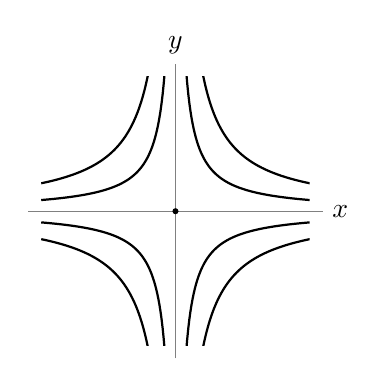
\begin{tikzpicture}[scale=0.55]
    % Coordinate axes
    \draw[gray] (-3.4,0) -- (3.4,0)
        node[right,black] {$x$};
    \draw[gray] (0,-3.4) -- (0,3.4)
        node[above,black] {$y$};

    % Curved trajectories: y=C/x
    \begin{scope}
        \clip (-3.1,-3.1) rectangle (3.1,3.1);
        \foreach \C in {-2,-0.8,0.8,2}{
            \draw[thick,domain=0.12:3.1,samples=120]
                plot (\x,{\C/\x});
            \draw[thick,domain=-3.1:-0.12,samples=120]
                plot (\x,{\C/\x});
        }
    \end{scope}
    % Equilibrium
    \fill (0,0) circle (2pt);
\end{tikzpicture}

\small
Curves move toward the origin and then bend away.
\end{minipage}
\hfill
%-------------------- Node --------------------
\begin{minipage}[t]{0.48\linewidth}
\centering
\textbf{Node}

\medskip
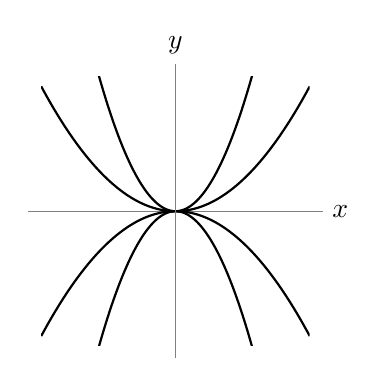
\begin{tikzpicture}[scale=0.55]
    % Coordinate axes
    \draw[gray] (-3.4,0) -- (3.4,0)
        node[right,black] {$x$};
    \draw[gray] (0,-3.4) -- (0,3.4)
        node[above,black] {$y$};

    % Curved trajectories: y=Cx^2
    % The two halves are separate trajectories.
    \begin{scope}
        \clip (-3.1,-3.1) rectangle (3.1,3.1);
        \foreach \C in {-1,-0.3,0.3,1}{
            \draw[thick,domain=0.02:3.1,samples=120]
                plot (\x,{\C*\x*\x});
            \draw[thick,domain=-3.1:-0.02,samples=120]
                plot (\x,{\C*\x*\x});
        }
    \end{scope}
\end{tikzpicture}

\small
Curved paths are tangent to one eigenvector line at the origin in the limit.
\end{minipage}
\end{center}


% SIDE NOTE: 9:18 | Name the stability we can now see
% a) Stable means stay close; asymptotically stable also means converge.
% b) Inward nodes are asymptotically stable; outward nodes and saddles are unstable.
% c) Skip marble analogies; use the phase portraits already on the board.
\section{Equilibrium Points and Stability}

\subsection{Equilibrium Points}

Consider the system
\[
\mathbf{x}'=A\mathbf{x}.
\]
Think of $\mathbf{x}(t)$ as the position of a particle.
An \textbf{equilibrium point} is a position
$\mathbf{x}_*$ where the particle remains at rest:
\[
\boxed{A\mathbf{x}_*=\mathbf{0}.}
\]
Starting at this point gives the constant solution
$\mathbf{x}(t)=\mathbf{x}_*$.

The origin is always an equilibrium. If $A$ is
nonsingular, it is the only equilibrium because
$A\mathbf{x}_*=\mathbf{0}$ has only the trivial solution.

%-------------------------------------------------------------
\subsection{Stability}

A \textbf{perturbation} is a small change in the
initial position. We classify an equilibrium by
what happens to nearby solutions:
\begin{itemize}
    \item \textbf{Stable}: solutions starting sufficiently
    close remain close for all future time.

    \item \textbf{Asymptotically stable}: the equilibrium
    is stable, and nearby solutions also converge to it.

    \item \textbf{Unstable}: some solutions starting
    arbitrarily close eventually move away.
\end{itemize}


%-------------------------------------------------------------

An inward node is \textbf{asymptotically stable}, often called a
\textbf{stable node}. An outward node is an \textbf{unstable node}.
A saddle is \textbf{unstable}: initial points arbitrarily close to the
origin on an outward linear orbit eventually leave its neighborhood.
Having an inward direction is not enough for stability.

\section{Nodes with Tilted Eigenvector Lines}

% SIDE NOTE: 9:23 | Why the tangent is the slow direction
% a) Compare e^(-t) with e^(-2t) in Example 1.
% b) The term with λ closer to zero dominates near the origin.
% c) For outward nodes the smaller positive λ gives the tangent near the origin too.
\subsection{Slow and Fast Directions}

In Example 1, $e^{-2t}$ decays faster than $e^{-t}$. Along the
trajectory through $(1,1)$,
\[
\frac{y(t)}{x(t)}=e^{-t}\longrightarrow0.
\]
This explains the horizontal tangent near the origin.
The \textbf{slow direction} is the eigenvector direction whose exponential
changes more slowly; the other is the \textbf{fast direction}.

Suppose
\[
0>\lambda_1>\lambda_2.
\]
Then $\lambda_1$ is closer to zero, so
$e^{\lambda_1t}$ decays more slowly than
$e^{\lambda_2t}$.

For a trajectory containing both components,
\[
\mathbf{x}(t)
=c_1e^{\lambda_1t}\mathbf{v}_1
+c_2e^{\lambda_2t}\mathbf{v}_2,
\qquad c_1c_2\ne0,
\]
we have:
\begin{itemize}
    \item As $t\to\infty$, the slower term
    $c_1e^{\lambda_1t}\mathbf{v}_1$ dominates.
    The trajectory approaches the origin tangent
    to the $\mathbf{v}_1$ line.

    \item As $t\to-\infty$, the faster term
    $c_2e^{\lambda_2t}\mathbf{v}_2$ dominates.
    Far from the origin, the trajectory's direction
    approaches the $\mathbf{v}_2$ line.
\end{itemize}

For sketching, remember:
\[
\text{Near the origin: tangent to the slow eigenvector line.}
\]
For a stable node, the slow eigenvalue is the one closest to zero.
For an outward node, curved trajectories are also tangent near the origin
to the eigenvector line with smaller $|\lambda|$, now as $t\to-\infty$.
The linear orbits themselves remain on their own eigenvector lines.
Far away, approaching the fast direction does not mean that the
fast eigenvector line is a straight-line asymptote.

%-------------------------------------------------------------

% SIDE NOTE: 9:27 | One tilted node
% a) Draw and orient the two lines quickly.
% b) Identify λ = -1 as the slow direction, then add the curves.
% c) Mark (3,-1) qualitatively; skip solving for constants. Start the zero eigenvalue by 9:34.
\begin{example}[2]{
Sketch the phase portrait for
\[
\mathbf{x}(t)
=c_1e^{-3t}\begin{pmatrix}1\\-1\end{pmatrix}
+c_2e^{-t}\begin{pmatrix}4\\1\end{pmatrix}.
\]
Label the trajectory satisfying
\[
\mathbf{x}(0)=\begin{pmatrix}3\\-1\end{pmatrix}.
\]
}

\paragraph{Step 1. Draw the linear orbits.}
The eigenvector lines are
\[
y=-x,\qquad y=\frac14x.
\]
Both eigenvalues are negative, so all four arrows
point toward the origin.

\paragraph{Step 2. Identify the slow direction.}
The eigenvalue $-1$ is closer to zero than $-3$.
Thus, curved trajectories approach the origin
tangent to
\[
y=\frac14x.
\]
Farther away, they bend toward the direction
of $y=-x$.

\paragraph{Step 3. Mark the initial point.}
Plot $(3,-1)$ and sketch the trajectory through it.
A qualitative sketch does not require solving for the constants.
For reference, the highlighted exact curve uses $c_1=7/5$ and $c_2=2/5$.

\paragraph{Step 4. Classify the equilibrium.}
Both eigenvalues are negative, so
\[
\boxed{(0,0)\text{ is a stable node.}}
\]

\begin{center}
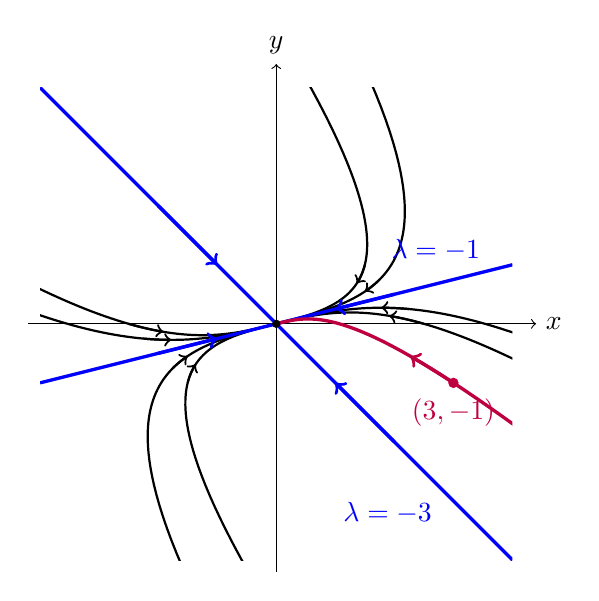
\begin{tikzpicture}[scale=0.75]
    \draw[->] (-4.2,0) -- (4.4,0) node[right] {$x$};
    \draw[->] (0,-4.2) -- (0,4.4) node[above] {$y$};

    \begin{scope}
        \clip (-4,-4) rectangle (4,4);

        \foreach \ca in {-0.5,-0.25,0.25,0.5}{
            \foreach \cb in {-0.5,0.5}{
                \draw[thick,domain=-1.2:5,
                      samples=250,variable=\t]
                    plot
                    ({\ca*exp(-3*\t)+4*\cb*exp(-\t)},
                     {-\ca*exp(-3*\t)+\cb*exp(-\t)});

                \draw[->,thick,domain=0:0.2,
                      samples=20,variable=\t]
                    plot
                    ({\ca*exp(-3*\t)+4*\cb*exp(-\t)},
                     {-\ca*exp(-3*\t)+\cb*exp(-\t)});
            }
        }

        \draw[blue,very thick] (-4,4) -- (4,-4);
        \draw[blue,very thick] (-4,-1) -- (4,1);
        \draw[->,blue,very thick] (2,-2) -- (1,-1);
        \draw[->,blue,very thick] (-2,2) -- (-1,1);
        \draw[->,blue,very thick] (2,0.5) -- (1,0.25);
        \draw[->,blue,very thick] (-2,-0.5) -- (-1,-0.25);

        \draw[purple,very thick,domain=-1:5,
              samples=250,variable=\t]
            plot
            ({(7/5)*exp(-3*\t)+(8/5)*exp(-\t)},
             {-(7/5)*exp(-3*\t)+(2/5)*exp(-\t)});

        \draw[->,purple,very thick,domain=0:0.15,
              samples=20,variable=\t]
            plot
            ({(7/5)*exp(-3*\t)+(8/5)*exp(-\t)},
             {-(7/5)*exp(-3*\t)+(2/5)*exp(-\t)});
    \end{scope}

    \fill[purple] (3,-1) circle (2.5pt);
    \node[purple,below] at (3,-1.1) {$(3,-1)$};
    \node[blue,above] at (2.7,0.9) {$\lambda=-1$};
    \node[blue,left] at (2.8,-3.2) {$\lambda=-3$};
    \fill (0,0) circle (2pt);
\end{tikzpicture}
\end{center}
\end{example}

%%%%%%%%%%%%%%%%%%%%%%%%%%%%%%%%%%%%%%%%%%%%%%%%%%%%%%%%%%%%%%%%%%%%%%%%

% SIDE NOTE: 9:34 | What changes when λ = 0?
% a) The zero-eigenvalue term is constant: a whole line of resting points.
% b) Other trajectories are shifted parallel rays, not curves between four rays.
% c) No motion arrows on the equilibrium line.
\section{A Line of Equilibria}

\subsection{A Zero Eigenvalue}

Suppose one eigenvalue is zero and the other is nonzero.
Then $A$ is singular, and
\[
A\mathbf{x}_*=\mathbf{0}
\]
has infinitely many solutions forming a line through
the origin. This is the \textbf{line of equilibria}.

If $\mathbf{v}_1$ is an eigenvector for $\lambda_1=0$,
then
\[
A\mathbf{v}_1=\mathbf{0}.
\]
Consequently, every point $c_1\mathbf{v}_1$ is an
equilibrium. The zero-eigenvalue eigenvector gives
the direction of the equilibrium line.

%-------------------------------------------------------------
\subsection{The Other Solution Curves}

With eigenvalues $0$ and $\lambda\ne0$, the general
solution is
\[
\boxed{
\mathbf{x}(t)
=c_1\mathbf{v}_1+c_2e^{\lambda t}\mathbf{v}_2.
}
\]
The first term is constant. It selects a point
$c_1\mathbf{v}_1$ on the line of equilibria.

The second term describes motion along a ray in
the $\mathbf{v}_2$ direction, shifted to that point.
Thus, the nonconstant trajectories are
\textbf{parallel rays}, each ending at or extending
away from a point on the equilibrium line.

The equilibrium point itself is not reached at
a finite time.

%-------------------------------------------------------------
\subsection{Sketching and Classification}

To sketch the phase portrait:
\begin{enumerate}
    \item Draw the line of equilibria in the
    $\mathbf{v}_1$ direction.
    \item Through several points on that line,
    draw lines parallel to $\mathbf{v}_2$.
    \item Treat the two sides of each equilibrium
    as separate trajectories.
    \item Add arrows using the nonzero eigenvalue:
    \[
    \lambda<0:\ \text{toward the equilibrium line},
    \qquad
    \lambda>0:\ \text{away from the equilibrium line}.
    \]
\end{enumerate}

The classification is
\[
\boxed{
\begin{array}{ll}
\lambda<0: & \text{stable line of equilibria},\\
\lambda>0: & \text{unstable line of equilibria}.
\end{array}
}
\]

For an attracting line, each equilibrium is stable but not asymptotically
stable. We will explain this distinction after the example.

%-------------------------------------------------------------

% SIDE NOTE: 9:39 | Sketch the line and shifted rays
% a) Use the supplied eigenpairs; no determinant expansion.
% b) Draw y = -x, then rays of slope -1/2 approaching it.
% c) Skip eliminating time if behind; use the vector form to explain the shift.
\begin{example}[3]{
Find the general solution, sketch the phase portrait,
and classify the equilibria:
\[
\mathbf{x}'=
\begin{pmatrix}
-2&-2\\
1&1
\end{pmatrix}\mathbf{x}.
\]
}

\paragraph{Step 1. Use the eigenpairs.}
The eigenpairs are
\[
\lambda_1=0,\quad \mathbf{v}_1=\begin{pmatrix}1\\-1\end{pmatrix},
\qquad
\lambda_2=-1,\quad \mathbf{v}_2=\begin{pmatrix}2\\-1\end{pmatrix}.
\]
Check them by multiplying $A\mathbf{v}_1=\mathbf{0}$ and
$A\mathbf{v}_2=-\mathbf{v}_2$. This leaves our attention on the sketch.

\paragraph{Step 2. Write the general solution.}
Since $e^{0t}=1$,
\[
\boxed{
\mathbf{x}(t)
=c_1\begin{pmatrix}1\\-1\end{pmatrix}
+c_2e^{-t}\begin{pmatrix}2\\-1\end{pmatrix}.
}
\]

\paragraph{Step 3. Sketch the phase portrait.}
The line of equilibria is
\[
y=-x.
\]
Other trajectories are parallel to
$\mathbf{v}_2=\begin{pmatrix}2\\-1\end{pmatrix}$,
so they lie on lines of slope $-1/2$.

Indeed,
\[
x=c_1+2c_2e^{-t},
\qquad
y=-c_1-c_2e^{-t},
\]
which gives
\[
y=-\frac12x-\frac12c_1.
\]
Each such line meets the equilibrium line at
$(c_1,-c_1)$. Since $\lambda_2=-1<0$, arrows point
toward that equilibrium from both sides.

\paragraph{Step 4. Classify the equilibria.}
\[
\boxed{y=-x\text{ is a stable line of equilibria.}}
\]

\begin{center}
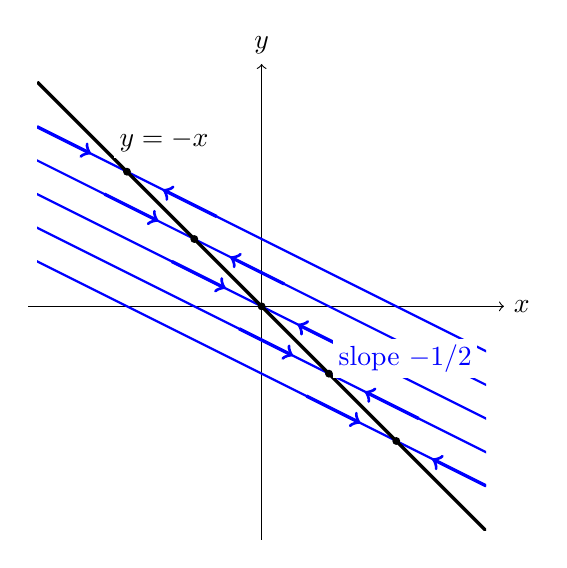
\begin{tikzpicture}[scale=0.57]
    \draw[->] (-5.2,0) -- (5.4,0) node[right] {$x$};
    \draw[->] (0,-5.2) -- (0,5.4) node[above] {$y$};

    \begin{scope}
        \clip (-5,-5) rectangle (5,5);

        % Each equilibrium is (b,-b).
        % Trajectories are parallel to (2,-1).
        \foreach \bb in {-3,-1.5,0,1.5,3}{
            \draw[blue,thick]
                ({\bb-12},{-\bb+6})
                --
                ({\bb+12},{-\bb-6});

            % Arrows toward the equilibrium from both sides.
            \draw[->,blue,very thick]
                ({\bb+2},{-\bb-1})
                --
                ({\bb+0.8},{-\bb-0.4});

            \draw[->,blue,very thick]
                ({\bb-2},{-\bb+1})
                --
                ({\bb-0.8},{-\bb+0.4});
        }

        \draw[black,very thick] (-5,5) -- (5,-5);
    \end{scope}

    \foreach \bb in {-3,-1.5,0,1.5,3}
        \fill[black] (\bb,{-\bb}) circle (2.5pt);

    \node[black,above right,fill=white,inner sep=2pt]
        at (-3.3,3.3) {$y=-x$};

    \node[blue,above,fill=white,inner sep=2pt]
        at (3.2,-1.6) {slope $-1/2$};
\end{tikzpicture}

\small
Each black point is an equilibrium. Blue trajectories
approach the equilibrium line without crossing it.
\end{center}
\end{example}


% SIDE NOTE: 9:46 | Stability of individual points on the line
% a) Nearby solutions approach some equilibrium, not necessarily the starting one.
% b) A point on an attracting line is stable but not asymptotically stable.
% c) Reverse the nonzero eigenvalue sign verbally to get a repelling line.

\clearpage
\subsection{Why Not Asymptotically Stable?}
In Example 3,
\[
\mathbf{x}(t)\longrightarrow c_1\begin{pmatrix}1\\-1\end{pmatrix}.
\]
The limiting equilibrium depends on the initial condition. A small
shift along $y=-x$ gives a different equilibrium that stays at rest.
Thus each point on this line is \textbf{stable but not asymptotically stable}.
Changing $A$ to $-A$ reverses the motion on the same rays: the line
then consists of unstable equilibria.


% SIDE NOTE: 9:49 | Exit check
% a) Opposite signs: saddle. Same nonzero sign: node. One zero: line of equilibria.
% b) Ask which eigenvector controls the node tangent near the origin.
% c) Finish at 9:50. If behind, omit the comparison pictures and exact-curve algebra, not the line example.

\begin{samepage}
\section{Summary}
For two distinct real eigenvalues:
\begin{center}
\begin{tabular}{c|l|l}
Eigenvalues & Portrait & Stability\\\hline
Opposite signs & Saddle & Unstable\\
Both negative & Inward node & Asymptotically stable\\
Both positive & Outward node & Unstable\\
Zero and negative & Line of equilibria & Stable, not asymptotically stable\\
Zero and positive & Line of equilibria & Unstable
\end{tabular}
\end{center}
In the last two rows, stability describes each individual equilibrium.
\end{samepage}
\end{document}

